\section{Experimental results\label{section:results}}


% \begin{figure}[h!]
% \begin{center}
%  \includegraphics[width=1\linewidth]{Grid_generation.png}
% \end{center}
% \end{figure}
\noindent
In this section, we discuss the experimental results obtained testing the formulations presented in Section \ref{Form} and the matheuristic procedure proposed in Section \ref{Math} on a testbed of instances. In particular, we consider instances like the ones used in \cite{art:Amorosi2021}, where the targets to be visited by the drones are represented by grid graphs.
We generated one set of 5 instances with 5 graphs and another set of 5 instances with 10 graphs. More precisely, each instance is composed of 20$\%$ graphs with 4 nodes, 20$\%$ graphs of 6 nodes, 20$\%$ graphs of 8 nodes, 20$\%$ graphs of 10 nodes and and 20$\%$ graphs with 12 nodes. Moreover, we assume that the velocity of the drones is twice that of the mothership and that a random fraction of each target graph, or of each of its edges, must be visited by the fleet of drones. These fractions are uniform\EN{ly} randomly sampled in the interval $(0, 1)$.\\

\noindent
%\subsection{ADD TITLE TO THE FIRST EXPERIMENT}} 
We consider in our experiments that the number of drones varies between 1 and 3 and that the drone endurance (expressed as the maximum time that the drone can operate when it is fully recharged) ranges between 20 and 60. Note that the case of a single drone is also included in our experiments to compare the results and complexity of using one \EN{or} more than one drone. The interested reader is referred to \cite{art:Amorosi2021} \EN{to analyze} the complexity in terms of gap of the model with a single drone.
Table \ref{table:tab1} reports a summary of the characteristics of our instances.

\renewcommand{\arraystretch}{0.7}
\begin{table}[!h]
\caption{Instance parameter values}
\centering
\footnotesize
\begin{tabular}{c | c }
\hline
$|\mathcal G|$ & (5,10)\\
\hline
$|\mathcal D|$ &	(1,2,3)\\
\hline
$|V_g|$ & (4,6,8,10,12)\\
\hline
$N_D$ & (20,30,40,50,60)\\
\hline
fraction target (edge) & uniform\EN{ly} randomly sampled in $(0, 1)$.
\end{tabular}
\label{table:tab1}
\end{table}

\noindent
We coded the matheuristic and the exact resolution of the model in Python 3.8.10. The mathematical programming formulation \EN{was} implemented in Gurobi 9.1.2. All the tests \EN{were} run on a machine AMD® Epyc 7402p with 24-core processor × 8.
Table \ref{table:tab2} reports the results obtained solving both variants of the \AMD\xspace model on the instances previously described, by adopting the commercial solver Gurobi. We consider the exact solution both providing and not providing an initial solution computed by the matheuristic described in Section \ref{Math}. More precisely, the first row of Table \ref{table:tab2} indicates the model variant and the second row reports the number of target graphs to be visited by the fleet of drones (5 or 10). From the third row, we split each column in\EN{to} three sub-columns. The first three sub-columns report respectively, the endurance of the drones, the size of the fleet of drones and \EN{an} indication \EN{of} the visit of a fraction of each edge (e) or a fraction of each target graph (g). From sub-column 4 to sub-column 15, we report, for each combination of the listed parameters characterizing the instances, respectively, the average gap without initialization by the solution provided by the matheuristic (wi), the average gap with initialization by the solution obtained by the matheuristic (i) and the solution time, in seconds, of the matheuristic (TimeH). The time limit of these experiments is set equal to 1 hour.\\
\noindent
We can observe that the value of the average percentage gap ranges between a minimum of 58\% and a maximum of 100\%. This shows that the model is hard \EN{to solve} even with small size instances. Moreover, we can see that for the complete overlapping version of the model, in most cases, the average gap associated with the variant of the model consisting \EN{of} visiting a given fraction of each edge, is higher than \EN{that} associated with the variant \EN{obligating} to visit a given fraction of each target graph. 
%The opposite behaviour can be observed for the partial overlapping version of the model.
Another thing that we can observe is that the average percentage gap increases with the number of target graphs for both problem variants.\\
\noindent
Moreover, the reader may note that the partial overlapping version of the problem is harder to solve than the complete overlapping version by looking at the values of the average gap. This is an expected \EN{behavior} due to the fact that the feasible region of the partial overlapping variant contains the one associated with the complete overlapping variant, as proven in Theorem \ref{th:relaxation}. 
We can see that for both versions of the problem, by increasing the number of target graphs from 5 to 10, the exact method without initialization of the solution obtained with the matheuristic, becomes even harder. Indeed, the gray entries of the table mean that some instances could not find a feasible solution within the time limit (note that in the brackets we indicate the number of these instances). %The number of not solved} instances increases with the number of drones.
\EN{Furthermore}, for the minimum level of endurance, the exact solution of the partial overlapping model without initialization provided by the matheuristic, does not find any solution within the time limit for instances with 10 graphs, 3 drones and a given fraction of each edge to be visited. The same can \EN{also} be observed for the exact solution of the complete overlapping model without initialization provided by the matheuristic, for a level of endurance equal to 30, a fleet of 3 drones and a given fraction of each edge to be visited.\\
Considering the comparison with the exact method starting from the solution provided by the matheuristic, we can note that the values of the average percentage gap are very close to \EN{those} related to the exact solution method without initialization. Thus, the initialization does not speed up the convergence of the solver. However, we can see that the matheuristic is always able to find a feasible solution \EN{to} the problem, even for the cases in which the solver is not. 

%INCLUDE EXPLANATION OF THE BOXPLOTS}
\noindent
Furthermore, the average solution times of the matheuristic range between a minimum of 4 seconds to a maximum of 9.5 minutes. In particular, we can observe that, in most cases, for the complete overlapping version of the problem, the matheuristic running time is shorter for the instances where a fraction of the length of each graph is required to be visited. The same \EN{behavior} can be noticed for the partial overlapping version of the problem for which the difference in terms of running time is even bigger. Indeed, when a given fraction of the length of each edge is required, STEP 1 of the matheuristic (computation of the TSP over the graph edges) takes more time. %They increase with the drone endurance} for the variant of the model in which a given fraction} of each edge must be visited, while they decrease by increasing the number of drones for the variant of the model in which a given fraction} of each target graph must be} visited. 
By increasing the number of target graphs from 5 to 10, the average solution times of the matheuristic increases for both model variants.
Summing up, the results obtained show that the exact solution method given by solving the formulation is very challenging even for small size instances. However, exploiting it, the matheuristic is able to provide  solutions for all instances \EN{quite} quickly.
% Please add the following required packages to your document preamble:
% Table generated by Excel2LaTeX from sheet 'Hoja2'
\begin{table}[h!]
  \centering
  \caption{Comparison between the partial and complete overlapping models}}
    \resizebox{\textwidth}{!}{
    \begin{tabular}{|c|c|c||ccc|ccc||ccc|ccc|}
    \hline
    \multicolumn{3}{|c|}{\textbf{Model}} & \multicolumn{6}{c|}{Complete Overlapping}     & \multicolumn{6}{c|}{Partial Overlapping} \bigstrut\\
    \hline
    \multicolumn{3}{|c|}{$|\mathcal G|$} & \multicolumn{3}{c|}{5} & \multicolumn{3}{c|}{10} & \multicolumn{3}{c|}{5} & \multicolumn{3}{c|}{10} \bigstrut\\
    \hline
    $N_D$ & $|\mathcal D|$ & $\alpha$ & Gap (wi) & Gap (i) & TimeH & Gap (wi) & Gap (i) & TimeH & Gap (wi) & Gap (i) & TimeH & Gap (wi) & Gap (i) & TimeH \bigstrut\\
    \hline
    \hline
    \multirow{6}[6]{*}{20} & \multirow{2}[2]{*}{1} & g     & 0.78  & 0.79  & 6.01  & \textcolor[rgb]{ 1,  0,  0}{0.91 (2)} & 0.86  & 177.69 & 0.65  & 0.63  & 16.53 & 1     & 1     & 215.59 \bigstrut[t]\\
          &       & e     & 0.81  & 0.81  & 15.41 & \textcolor[rgb]{ 1,  0,  0}{0.89 (2)} & 0.84  & 148.95 & 0.84  & 0.83  & 52.36 & \textcolor[rgb]{ 1,  0,  0}{0.88 (3)} & 0.87  & 440.93 \bigstrut[b]\\
\cline{2-15}          & \multirow{2}[2]{*}{2} & g     & 0.81  & 0.87  & 5.76  & \textcolor[rgb]{ 1,  0,  0}{0.96 (3)} & 0.96  & 139.24 & 0.97  & 0.96  & 13.91 & \textcolor[rgb]{ 1,  0,  0}{1 (3)} & 1     & 76.77 \bigstrut[t]\\
          &       & e     & 0.93  & 0.92  & 33.99 & \textcolor[rgb]{ 1,  0,  0}{0.97 (3)} & 0.97  & 163.41 & \textcolor[rgb]{ 1,  0,  0}{0.86 (2)} & 0.85  & 66.38 & \textcolor[rgb]{ 1,  0,  0}{0.89 (4)} & 0.85  & 578.31 \bigstrut[b]\\
\cline{2-15}          & \multirow{2}[2]{*}{3} & g     & 0.88  & 0.89  & 4.83  & \textcolor[rgb]{ 1,  0,  0}{0.95 (3)} & 0.94  & 67.76 & 0.97  & 0.97  & 17.87 & \textcolor[rgb]{ 1,  0,  0}{1 (2)} & 1     & 18.88 \bigstrut[t]\\
          &       & e     & 0.92  & 0.91  & 14.08 & \textcolor[rgb]{ 1,  0,  0}{0.97 (2)} & 0.97  & 125.89 & \textcolor[rgb]{ 1,  0,  0}{0.81 (3)} & 0.84  & 61.83 & \textcolor[rgb]{ 1,  0,  0}{- (5)} & 0.82  & 237.33 \bigstrut[b]\\
    \hline
    \hline
    \multirow{6}[6]{*}{30} & \multirow{2}[2]{*}{1} & g     & 0.71  & 0.7   & 9.66  & \textcolor[rgb]{ 1,  0,  0}{0.82 (4)} & 0.82  & 87.4  & 0.77  & 0.75  & 15.43 & 1     & 1     & 39.83 \bigstrut[t]\\
          &       & e     & 0.79  & 0.8   & 14.16 & \textcolor[rgb]{ 1,  0,  0}{0.8 (4)} & 0.83  & 122.23 & 0.84  & 0.82  & 38.94 & \textcolor[rgb]{ 1,  0,  0}{0.83 (4)} & 0.81  & 289.74 \bigstrut[b]\\
\cline{2-15}          & \multirow{2}[2]{*}{2} & g     & 0.82  & 0.82  & 4.98  & \textcolor[rgb]{ 1,  0,  0}{0.95 (3)} & 0.92  & 174.64 & 0.97  & 0.96  & 12.94 & 1     & 1     & 45.37 \bigstrut[t]\\
          &       & e     & 0.84  & 0.84  & 14.73 & \textcolor[rgb]{ 1,  0,  0}{0.96 (3)} & 0.97  & 133.75 & 0.78  & 0.79  & 31.82 & 0.82  & 0.77  & 171.16 \bigstrut[b]\\
\cline{2-15}          & \multirow{2}[2]{*}{3} & g     & 0.82  & 0.81  & 4.63  & \textcolor[rgb]{ 1,  0,  0}{0.93 (3)} & 0.95  & 105.54 & 0.96  & 0.96  & 16.22 & 1     & 1     & 33.95 \bigstrut[t]\\
          &       & e     & 0.88  & 0.89  & 12.08 & \textcolor[rgb]{ 1,  0,  0}{- (5)} & 0.97  & 127.78 & 0.83  & 0.82  & 35.38 & \textcolor[rgb]{ 1,  0,  0}{0.79 (3)} & 0.8   & 213.06 \bigstrut[b]\\
    \hline
    \hline
    \multirow{6}[6]{*}{40} & \multirow{2}[2]{*}{1} & g     & 0.68  & 0.68  & 5.79  & \textcolor[rgb]{ 1,  0,  0}{0.81 (2)} & 0.82  & 93.21 & 0.73  & 0.71  & 11.46 & 1     & 1     & 48.85 \bigstrut[t]\\
          &       & e     & 0.76  & 0.77  & 37.55 & \textcolor[rgb]{ 1,  0,  0}{0.78 (4)} & 0.81  & 160.24 & 0.8   & 0.79  & 57.28 & \textcolor[rgb]{ 1,  0,  0}{0.79 (1)} & 0.8   & 403.72 \bigstrut[b]\\
\cline{2-15}          & \multirow{2}[2]{*}{2} & g     & 0.72  & 0.66  & 5.14  & \textcolor[rgb]{ 1,  0,  0}{0.91 (2)} & 0.92  & 131.26 & 0.96  & 0.95  & 11.48 & 1     & 1     & 35.71 \bigstrut[t]\\
          &       & e     & 0.83  & 0.78  & 19.46 & \textcolor[rgb]{ 1,  0,  0}{0.91 (2)} & 0.95  & 141.6 & 0.79  & 0.79  & 35.79 & \textcolor[rgb]{ 1,  0,  0}{0.79 (1)} & 0.79  & 576.75 \bigstrut[b]\\
\cline{2-15}          & \multirow{2}[2]{*}{3} & g     & 0.61  & 0.62  & 3.91  & 0.91  & 0.91  & 115.48 & 0.95  & 0.95  & 15.13 & 1     & 1     & 17.98 \bigstrut[t]\\
          &       & e     & 0.85  & 0.83  & 15.36 & 0.93  & 0.94  & 85.9  & 0.81  & 0.81  & 40.37 & \textcolor[rgb]{ 1,  0,  0}{0.81 (1)} & 0.8   & 309.09 \bigstrut[b]\\
    \hline
    \hline
    \multirow{6}[6]{*}{50} & \multirow{2}[2]{*}{1} & g     & 0.65  & 0.64  & 5.52  & \textcolor[rgb]{ 1,  0,  0}{0.82 (3)} & 0.84  & 101.24 & 0.82  & 0.78  & 9.53  & 1     & 1     & 32.54 \bigstrut[t]\\
          &       & e     & 0.74  & 0.73  & 16.63 & \textcolor[rgb]{ 1,  0,  0}{0.81 (3)} & 0.83  & 118.67 & 0.78  & 0.77  & 58.95 & \textcolor[rgb]{ 1,  0,  0}{0.82 (2)} & 0.82  & 311.02 \bigstrut[b]\\
\cline{2-15}          & \multirow{2}[2]{*}{2} & g     & 0.7   & 0.7   & 6.37  & \textcolor[rgb]{ 1,  0,  0}{0.9 (1)} & 0.93  & 206.87 & 0.97  & 0.97  & 14.68 & 1     & 1     & 39.5 \bigstrut[t]\\
          &       & e     & 0.67  & 0.73  & 12.07 & \textcolor[rgb]{ 1,  0,  0}{0.92 (2)} & 0.93  & 168.57 & 0.77  & 0.77  & 36.46 & \textcolor[rgb]{ 1,  0,  0}{0.8 (1)} & 0.81  & 265.16 \bigstrut[b]\\
\cline{2-15}          & \multirow{2}[2]{*}{3} & g     & 0.65  & 0.64  & 4.27  & \textcolor[rgb]{ 1,  0,  0}{0.9 (1)} & 0.93  & 26.68 & 0.94  & 0.92  & 19.08 & 1     & 1     & 15.97 \bigstrut[t]\\
          &       & e     & 0.74  & 0.74  & 12.95 & 0.9   & 0.94  & 90.14 & 0.8   & 0.79  & 40.77 & \textcolor[rgb]{ 1,  0,  0}{0.76 (3)} & 0.79  & 195.68 \bigstrut[b]\\
    \hline
    \hline
    \multirow{6}[6]{*}{60} & \multirow{2}[2]{*}{1} & g     & 0.69  & 0.7   & 5.58  & \textcolor[rgb]{ 1,  0,  0}{0.8 (4)} & 0.81  & 83.02 & 0.78  & 0.76  & 11.18 & 1     & 1     & 36.78 \bigstrut[t]\\
          &       & e     & 0.74  & 0.74  & 16.53 & \textcolor[rgb]{ 1,  0,  0}{0.85 (2)} & 0.86  & 145.06 & 0.76  & 0.76  & 37.73 & \textcolor[rgb]{ 1,  0,  0}{0.84 (2)} & 0.83  & 359.68 \bigstrut[b]\\
\cline{2-15}          & \multirow{2}[2]{*}{2} & g     & 0.67  & 0.72  & 4.09  & \textcolor[rgb]{ 1,  0,  0}{0.94 (2)} & 0.94  & 81.69 & 0.95  & 0.94  & 13.33 & 1     & 1     & 17.04 \bigstrut[t]\\
          &       & e     & 0.76  & 0.73  & 15.58 & \textcolor[rgb]{ 1,  0,  0}{0.94 (2)} & 0.92  & 108.17 & 0.78  & 0.78  & 33.28 & 0.78  & 0.79  & 237.38 \bigstrut[b]\\
\cline{2-15}          & \multirow{2}[2]{*}{3} & g     & 0.58  & 0.53  & 7     & \textcolor[rgb]{ 1,  0,  0}{0.89 (2)} & 0.9   & 60.99 & 0.91  & 0.94  & 20.15 & 1     & 1     & 33.93 \bigstrut[t]\\
          &       & e     & 0.72  & 0.7   & 15.39 & \textcolor[rgb]{ 1,  0,  0}{0.91 (2)} & 0.96  & 96.52 & 0.78  & 0.78  & 49.39 & 0.81  & 0.81  & 259.34 \bigstrut[b]\\
    \hline
    \end{tabular}}%
  \label{table:tab2}%
\end{table}%

\noindent
The boxplots in Figure \ref{fig:gap_boxplot_synchronous}  represent the relative gap of the solution provided by the matheuristic for the complete overlapping version of the problem, with respect to \EN{that} provided by the exact solution of the mathematical programming model within the time limit, with the initialization of the solution found by the matheuristic. Similarly, Figure \ref{fig:gap_boxplot_asynchronous} reports the same information for the partial overlapping version of the problem.

% This file was created with tikzplotlib v0.9.12.
\definecolor{color0}{rgb}{0.917647058823529,0.917647058823529,0.949019607843137}
\definecolor{color1}{rgb}{0.347058823529412,0.458823529411765,0.641176470588235}
\definecolor{color2}{rgb}{0.798529411764706,0.536764705882353,0.389705882352941}

\begin{figure}[h!]
\centering
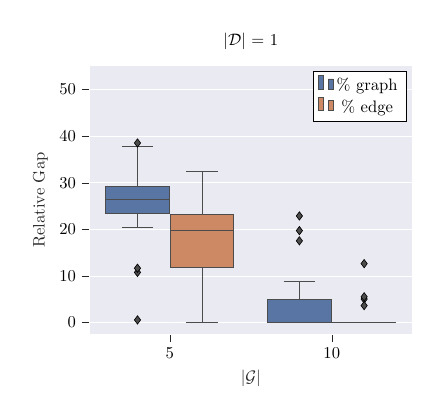
\begin{tikzpicture}[scale=0.6]

\begin{axis}[
axis background/.style={fill=color0},
axis line style={white},
tick align=outside,
title={$|\mathcal D|$ = 1},
x grid style={white},
xlabel=\textcolor{white!15!black}{$|\mathcal G|$},
xtick pos = left,
ytick pos = left,
xmin=-0.5, xmax=1.5,
xtick style={color=white!15!black},
xtick={0,1},
xticklabels={5,10},
y grid style={white},
ylabel=\textcolor{white!15!black}{Relative Gap},
ymajorgrids,
ymin=-2.62609180192484, ymax=55.1479278404217,
ytick style={color=white!15!black}
]
\path [draw=white!29.8039215686275!black, fill=color1, semithick]
(axis cs:-0.396,23.351171126429)
--(axis cs:-0.004,23.351171126429)
--(axis cs:-0.004,29.1428581886508)
--(axis cs:-0.396,29.1428581886508)
--(axis cs:-0.396,23.351171126429)
--cycle;
\path [draw=white!29.8039215686275!black, fill=color2, semithick]
(axis cs:0.004,11.7176590067474)
--(axis cs:0.396,11.7176590067474)
--(axis cs:0.396,23.2397374756161)
--(axis cs:0.004,23.2397374756161)
--(axis cs:0.004,11.7176590067474)
--cycle;
\path [draw=white!29.8039215686275!black, fill=color1, semithick]
(axis cs:0.604,0)
--(axis cs:0.996,0)
--(axis cs:0.996,4.91567244371752)
--(axis cs:0.604,4.91567244371752)
--(axis cs:0.604,0)
--cycle;
\path [draw=white!29.8039215686275!black, fill=color2, semithick]
(axis cs:1.004,0)
--(axis cs:1.396,0)
--(axis cs:1.396,0)
--(axis cs:1.004,0)
--(axis cs:1.004,0)
--cycle;
\draw[draw=white!29.8039215686275!black,fill=color1,line width=0.3pt] (axis cs:0,0) rectangle (axis cs:0,0);
\addlegendimage{ybar,ybar legend,draw=white!29.8039215686275!black,fill=color1,line width=0.3pt}
\addlegendentry{\% graph}

\draw[draw=white!29.8039215686275!black,fill=color2,line width=0.3pt] (axis cs:0,0) rectangle (axis cs:0,0);
\addlegendimage{ybar,ybar legend,draw=white!29.8039215686275!black,fill=color2,line width=0.3pt}
\addlegendentry{\% edge}

\addplot [semithick, white!29.8039215686275!black]
table {%
-0.2 23.351171126429
-0.2 20.2948309102868
};
\addplot [semithick, white!29.8039215686275!black]
table {%
-0.2 29.1428581886508
-0.2 37.7174995502607
};
\addplot [semithick, white!29.8039215686275!black]
table {%
-0.298 20.2948309102868
-0.102 20.2948309102868
};
\addplot [semithick, white!29.8039215686275!black]
table {%
-0.298 37.7174995502607
-0.102 37.7174995502607
};
\addplot [black, mark=diamond*, mark size=2.5, mark options={solid,fill=white!29.8039215686275!black}, only marks]
table {%
-0.2 10.7436731274202
-0.2 0.532520584131128
-0.2 11.63870481964
-0.2 38.5383150484397
};
\addplot [semithick, white!29.8039215686275!black]
table {%
0.2 11.7176590067474
0.2 0
};
\addplot [semithick, white!29.8039215686275!black]
table {%
0.2 23.2397374756161
0.2 32.3710612542474
};
\addplot [semithick, white!29.8039215686275!black]
table {%
0.102 0
0.298 0
};
\addplot [semithick, white!29.8039215686275!black]
table {%
0.102 32.3710612542474
0.298 32.3710612542474
};
\addplot [semithick, white!29.8039215686275!black]
table {%
0.8 0
0.8 0
};
\addplot [semithick, white!29.8039215686275!black]
table {%
0.8 4.91567244371752
0.8 8.74627321462437
};
\addplot [semithick, white!29.8039215686275!black]
table {%
0.702 0
0.898 0
};
\addplot [semithick, white!29.8039215686275!black]
table {%
0.702 8.74627321462437
0.898 8.74627321462437
};
\addplot [black, mark=diamond*, mark size=2.5, mark options={solid,fill=white!29.8039215686275!black}, only marks]
table {%
0.8 19.7135319472805
0.8 22.8600948091405
0.8 17.5254820302641
};
\addplot [semithick, white!29.8039215686275!black]
table {%
1.2 0
1.2 0
};
\addplot [semithick, white!29.8039215686275!black]
table {%
1.2 0
1.2 0
};
\addplot [semithick, white!29.8039215686275!black]
table {%
1.102 0
1.298 0
};
\addplot [semithick, white!29.8039215686275!black]
table {%
1.102 0
1.298 0
};
\addplot [black, mark=diamond*, mark size=2.5, mark options={solid,fill=white!29.8039215686275!black}, only marks]
table {%
1.2 5.01285212584406
1.2 12.6187782464826
1.2 3.60850467468294
1.2 5.50654876776942
};
\addplot [semithick, white!29.8039215686275!black]
table {%
-0.396 26.3941988580451
-0.004 26.3941988580451
};
\addplot [semithick, white!29.8039215686275!black]
table {%
0.004 19.8419895666702
0.396 19.8419895666702
};
\addplot [semithick, white!29.8039215686275!black]
table {%
0.604 0
0.996 0
};
\addplot [semithick, white!29.8039215686275!black]
table {%
1.004 0
1.396 0
};
\end{axis}
\end{tikzpicture}
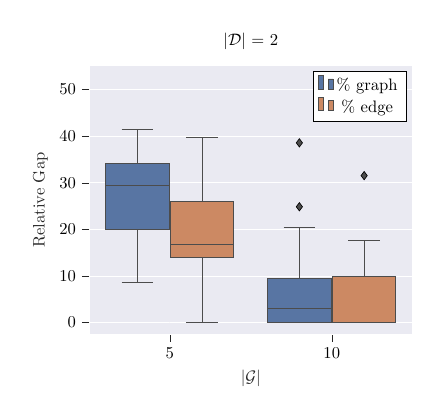
\begin{tikzpicture}[scale = 0.6]
\begin{axis}[
axis background/.style={fill=color0},
axis line style={white},
tick align=outside,
title={$|\mathcal D|$ = 2},
x grid style={white},
xlabel=\textcolor{white!15!black}{$|\mathcal G|$},
xtick pos = left,
ytick pos = left,
xmin=-0.5, xmax=1.5,
xtick style={color=white!15!black},
xtick={0,1},
xticklabels={5,10},
y grid style={white},
ylabel=\textcolor{white!15!black}{Relative Gap},
ymajorgrids,
ymin=-2.62609180192484, ymax=55.1479278404217,
ytick style={color=white!15!black}
]
\path [draw=white!29.8039215686275!black, fill=color1, semithick]
(axis cs:-0.396,19.9290413160217)
--(axis cs:-0.004,19.9290413160217)
--(axis cs:-0.004,34.1534565237393)
--(axis cs:-0.396,34.1534565237393)
--(axis cs:-0.396,19.9290413160217)
--cycle;
\path [draw=white!29.8039215686275!black, fill=color2, semithick]
(axis cs:0.004,13.8445034768791)
--(axis cs:0.396,13.8445034768791)
--(axis cs:0.396,25.9198033064554)
--(axis cs:0.004,25.9198033064554)
--(axis cs:0.004,13.8445034768791)
--cycle;
\path [draw=white!29.8039215686275!black, fill=color1, semithick]
(axis cs:0.604,0)
--(axis cs:0.996,0)
--(axis cs:0.996,9.44492782733373)
--(axis cs:0.604,9.44492782733373)
--(axis cs:0.604,0)
--cycle;
\path [draw=white!29.8039215686275!black, fill=color2, semithick]
(axis cs:1.004,0)
--(axis cs:1.396,0)
--(axis cs:1.396,9.95730680242487)
--(axis cs:1.004,9.95730680242487)
--(axis cs:1.004,0)
--cycle;
\draw[draw=white!29.8039215686275!black,fill=color1,line width=0.3pt] (axis cs:0,0) rectangle (axis cs:0,0);
\addlegendimage{ybar,ybar legend,draw=white!29.8039215686275!black,fill=color1,line width=0.3pt}
\addlegendentry{\% graph}

\draw[draw=white!29.8039215686275!black,fill=color2,line width=0.3pt] (axis cs:0,0) rectangle (axis cs:0,0);
\addlegendimage{ybar,ybar legend,draw=white!29.8039215686275!black,fill=color2,line width=0.3pt}
\addlegendentry{\% edge}
\addplot [semithick, white!29.8039215686275!black]
table {%
-0.2 19.9290413160217
-0.2 8.56923471336534
};
\addplot [semithick, white!29.8039215686275!black]
table {%
-0.2 34.1534565237393
-0.2 41.461981811718
};
\addplot [semithick, white!29.8039215686275!black]
table {%
-0.298 8.56923471336534
-0.102 8.56923471336534
};
\addplot [semithick, white!29.8039215686275!black]
table {%
-0.298 41.461981811718
-0.102 41.461981811718
};
\addplot [semithick, white!29.8039215686275!black]
table {%
0.2 13.8445034768791
0.2 0
};
\addplot [semithick, white!29.8039215686275!black]
table {%
0.2 25.9198033064554
0.2 39.6956477504428
};
\addplot [semithick, white!29.8039215686275!black]
table {%
0.102 0
0.298 0
};
\addplot [semithick, white!29.8039215686275!black]
table {%
0.102 39.6956477504428
0.298 39.6956477504428
};
\addplot [semithick, white!29.8039215686275!black]
table {%
0.8 0
0.8 0
};
\addplot [semithick, white!29.8039215686275!black]
table {%
0.8 9.44492782733373
0.8 20.424957302526
};
\addplot [semithick, white!29.8039215686275!black]
table {%
0.702 0
0.898 0
};
\addplot [semithick, white!29.8039215686275!black]
table {%
0.702 20.424957302526
0.898 20.424957302526
};
\addplot [black, mark=diamond*, mark size=2.5, mark options={solid,fill=white!29.8039215686275!black}, only marks]
table {%
0.8 38.5697950554177
0.8 24.8433139698412
};
\addplot [semithick, white!29.8039215686275!black]
table {%
1.2 0
1.2 0
};
\addplot [semithick, white!29.8039215686275!black]
table {%
1.2 9.95730680242487
1.2 17.5555017835489
};
\addplot [semithick, white!29.8039215686275!black]
table {%
1.102 0
1.298 0
};
\addplot [semithick, white!29.8039215686275!black]
table {%
1.102 17.5555017835489
1.298 17.5555017835489
};
\addplot [black, mark=diamond*, mark size=2.5, mark options={solid,fill=white!29.8039215686275!black}, only marks]
table {%
1.2 31.522609110702
};
\addplot [semithick, white!29.8039215686275!black]
table {%
-0.396 29.4917032318658
-0.004 29.4917032318658
};
\addplot [semithick, white!29.8039215686275!black]
table {%
0.004 16.8115230551657
0.396 16.8115230551657
};
\addplot [semithick, white!29.8039215686275!black]
table {%
0.604 2.90644304969017
0.996 2.90644304969017
};
\addplot [semithick, white!29.8039215686275!black]
table {%
1.004 0
1.396 0
};
\end{axis}
\end{tikzpicture}
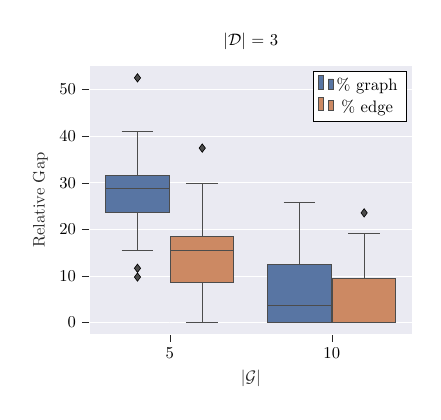
\begin{tikzpicture}[scale = 0.6]
\begin{axis}[
axis background/.style={fill=color0},
axis line style={white},
tick align=outside,
title={$|\mathcal D|$ = 3},
x grid style={white},
xlabel=\textcolor{white!15!black}{$|\mathcal G|$},
xtick pos = left,
ytick pos = left,
xmin=-0.5, xmax=1.5,
xtick style={color=white!15!black},
xtick={0,1},
xticklabels={5,10},
y grid style={white},
ylabel=\textcolor{white!15!black}{Relative Gap},
ymajorgrids,
ymin=-2.62609180192484, ymax=55.1479278404217,
ytick style={color=white!15!black}
]
\path [draw=white!29.8039215686275!black, fill=color1, semithick]
(axis cs:-0.396,23.6711838672955)
--(axis cs:-0.004,23.6711838672955)
--(axis cs:-0.004,31.6212153500762)
--(axis cs:-0.396,31.6212153500762)
--(axis cs:-0.396,23.6711838672955)
--cycle;
\path [draw=white!29.8039215686275!black, fill=color2, semithick]
(axis cs:0.004,8.46710294657892)
--(axis cs:0.396,8.46710294657892)
--(axis cs:0.396,18.4872052896899)
--(axis cs:0.004,18.4872052896899)
--(axis cs:0.004,8.46710294657892)
--cycle;
\path [draw=white!29.8039215686275!black, fill=color1, semithick]
(axis cs:0.604,0)
--(axis cs:0.996,0)
--(axis cs:0.996,12.5165770663005)
--(axis cs:0.604,12.5165770663005)
--(axis cs:0.604,0)
--cycle;
\path [draw=white!29.8039215686275!black, fill=color2, semithick]
(axis cs:1.004,0)
--(axis cs:1.396,0)
--(axis cs:1.396,9.35231931243425)
--(axis cs:1.004,9.35231931243425)
--(axis cs:1.004,0)
--cycle;
\draw[draw=white!29.8039215686275!black,fill=color1,line width=0.3pt] (axis cs:0,0) rectangle (axis cs:0,0);
\addlegendimage{ybar,ybar legend,draw=white!29.8039215686275!black,fill=color1,line width=0.3pt}
\addlegendentry{\% graph}

\draw[draw=white!29.8039215686275!black,fill=color2,line width=0.3pt] (axis cs:0,0) rectangle (axis cs:0,0);
\addlegendimage{ybar,ybar legend,draw=white!29.8039215686275!black,fill=color2,line width=0.3pt}
\addlegendentry{\% edge}
\addplot [semithick, white!29.8039215686275!black]
table {%
-0.2 23.6711838672955
-0.2 15.4058191019539
};
\addplot [semithick, white!29.8039215686275!black]
table {%
-0.2 31.6212153500762
-0.2 40.9222996550122
};
\addplot [semithick, white!29.8039215686275!black]
table {%
-0.298 15.4058191019539
-0.102 15.4058191019539
};
\addplot [semithick, white!29.8039215686275!black]
table {%
-0.298 40.9222996550122
-0.102 40.9222996550122
};
\addplot [black, mark=diamond*, mark size=2.5, mark options={solid,fill=white!29.8039215686275!black}, only marks]
table {%
-0.2 9.74044059855204
-0.2 11.6245127787016
-0.2 52.5218360384969
};
\addplot [semithick, white!29.8039215686275!black]
table {%
0.2 8.46710294657892
0.2 0
};
\addplot [semithick, white!29.8039215686275!black]
table {%
0.2 18.4872052896899
0.2 29.8677006223528
};
\addplot [semithick, white!29.8039215686275!black]
table {%
0.102 0
0.298 0
};
\addplot [semithick, white!29.8039215686275!black]
table {%
0.102 29.8677006223528
0.298 29.8677006223528
};
\addplot [black, mark=diamond*, mark size=2.5, mark options={solid,fill=white!29.8039215686275!black}, only marks]
table {%
0.2 37.4363390406919
};
\addplot [semithick, white!29.8039215686275!black]
table {%
0.8 0
0.8 0
};
\addplot [semithick, white!29.8039215686275!black]
table {%
0.8 12.5165770663005
0.8 25.7880376290282
};
\addplot [semithick, white!29.8039215686275!black]
table {%
0.702 0
0.898 0
};
\addplot [semithick, white!29.8039215686275!black]
table {%
0.702 25.7880376290282
0.898 25.7880376290282
};
\addplot [semithick, white!29.8039215686275!black]
table {%
1.2 0
1.2 0
};
\addplot [semithick, white!29.8039215686275!black]
table {%
1.2 9.35231931243425
1.2 19.1076748405332
};
\addplot [semithick, white!29.8039215686275!black]
table {%
1.102 0
1.298 0
};
\addplot [semithick, white!29.8039215686275!black]
table {%
1.102 19.1076748405332
1.298 19.1076748405332
};
\addplot [black, mark=diamond*, mark size=2.5, mark options={solid,fill=white!29.8039215686275!black}, only marks]
table {%
1.2 23.5231966348794
};
\addplot [semithick, white!29.8039215686275!black]
table {%
-0.396 28.7560216547077
-0.004 28.7560216547077
};
\addplot [semithick, white!29.8039215686275!black]
table {%
0.004 15.3383284127274
0.396 15.3383284127274
};
\addplot [semithick, white!29.8039215686275!black]
table {%
0.604 3.55548801271162
0.996 3.55548801271162
};
\addplot [semithick, white!29.8039215686275!black]
table {%
1.004 0
1.396 0
};
\end{axis}
\end{tikzpicture}
\caption{Relative gap boxplots for \AMDCO}
\label{fig:gap_boxplot_synchronous}
\end{figure}
% This file was created with tikzplotlib v0.9.16.
\begin{tikzpicture}

\definecolor{color0}{rgb}{0.917647058823529,0.917647058823529,0.949019607843137}
\definecolor{color1}{rgb}{0.347058823529412,0.458823529411765,0.641176470588235}
\definecolor{color2}{rgb}{0.798529411764706,0.536764705882353,0.389705882352941}

\begin{groupplot}[group style={group size=3 by 1}]
\nextgroupplot[
axis background/.style={fill=color0},
axis line style={white},
tick align=outside,
title={Num\_Drones = 1},
x grid style={white},
xlabel=\textcolor{white!15!black}{Size},
xmajorticks=false,
xmin=-0.5, xmax=1.5,
xtick style={color=white!15!black},
xtick={0,1},
xticklabels={5,10},
y grid style={white},
ylabel=\textcolor{white!15!black}{Difference},
ymajorgrids,
ymajorticks=false,
ymin=-2.78589617601925, ymax=58.5038196964039,
ytick style={color=white!15!black}
]
\path [draw=white!29.8039215686275!black, fill=color1, semithick]
(axis cs:-0.396,31.1204388239023)
--(axis cs:-0.004,31.1204388239023)
--(axis cs:-0.004,39.1875540319087)
--(axis cs:-0.396,39.1875540319087)
--(axis cs:-0.396,31.1204388239023)
--cycle;
\path [draw=white!29.8039215686275!black, fill=color2, semithick]
(axis cs:0.004,3.94465074664802)
--(axis cs:0.396,3.94465074664802)
--(axis cs:0.396,15.8590980671085)
--(axis cs:0.004,15.8590980671085)
--(axis cs:0.004,3.94465074664802)
--cycle;
\path [draw=white!29.8039215686275!black, fill=color1, semithick]
(axis cs:0.604,21.503687692433)
--(axis cs:0.996,21.503687692433)
--(axis cs:0.996,33.4822469494839)
--(axis cs:0.604,33.4822469494839)
--(axis cs:0.604,21.503687692433)
--cycle;
\path [draw=white!29.8039215686275!black, fill=color2, semithick]
(axis cs:1.004,0.0166178173158948)
--(axis cs:1.396,0.0166178173158948)
--(axis cs:1.396,9.65334660171153)
--(axis cs:1.004,9.65334660171153)
--(axis cs:1.004,0.0166178173158948)
--cycle;
\draw[draw=white!29.8039215686275!black,fill=color1,line width=0.3pt] (axis cs:0,0) rectangle (axis cs:0,0);
\addlegendimage{ybar,ybar legend,draw=white!29.8039215686275!black,fill=color1,line width=0.3pt}
\addlegendentry{False}

\draw[draw=white!29.8039215686275!black,fill=color2,line width=0.3pt] (axis cs:0,0) rectangle (axis cs:0,0);
\addlegendimage{ybar,ybar legend,draw=white!29.8039215686275!black,fill=color2,line width=0.3pt}
\addlegendentry{True}

\addplot [semithick, white!29.8039215686275!black]
table {%
-0.2 31.1204388239023
-0.2 23.0784232720862
};
\addplot [semithick, white!29.8039215686275!black]
table {%
-0.2 39.1875540319087
-0.2 50.257108804829
};
\addplot [semithick, white!29.8039215686275!black]
table {%
-0.298 23.0784232720862
-0.102 23.0784232720862
};
\addplot [semithick, white!29.8039215686275!black]
table {%
-0.298 50.257108804829
-0.102 50.257108804829
};
\addplot [semithick, white!29.8039215686275!black]
table {%
0.2 3.94465074664802
0.2 0
};
\addplot [semithick, white!29.8039215686275!black]
table {%
0.2 15.8590980671085
0.2 21.6662987917465
};
\addplot [semithick, white!29.8039215686275!black]
table {%
0.102 0
0.298 0
};
\addplot [semithick, white!29.8039215686275!black]
table {%
0.102 21.6662987917465
0.298 21.6662987917465
};
\addplot [semithick, white!29.8039215686275!black]
table {%
0.8 21.503687692433
0.8 8.42226170108821
};
\addplot [semithick, white!29.8039215686275!black]
table {%
0.8 33.4822469494839
0.8 43.749642590742
};
\addplot [semithick, white!29.8039215686275!black]
table {%
0.702 8.42226170108821
0.898 8.42226170108821
};
\addplot [semithick, white!29.8039215686275!black]
table {%
0.702 43.749642590742
0.898 43.749642590742
};
\addplot [semithick, white!29.8039215686275!black]
table {%
1.2 0.0166178173158948
1.2 -1.20043917969557e-14
};
\addplot [semithick, white!29.8039215686275!black]
table {%
1.2 9.65334660171153
1.2 20.5254784728402
};
\addplot [semithick, white!29.8039215686275!black]
table {%
1.102 -1.20043917969557e-14
1.298 -1.20043917969557e-14
};
\addplot [semithick, white!29.8039215686275!black]
table {%
1.102 20.5254784728402
1.298 20.5254784728402
};
\addplot [semithick, white!29.8039215686275!black]
table {%
-0.396 35.2275964209729
-0.004 35.2275964209729
};
\addplot [semithick, white!29.8039215686275!black]
table {%
0.004 9.56963060158162
0.396 9.56963060158162
};
\addplot [semithick, white!29.8039215686275!black]
table {%
0.604 28.9060977271458
0.996 28.9060977271458
};
\addplot [semithick, white!29.8039215686275!black]
table {%
1.004 0.0331954801373742
1.396 0.0331954801373742
};

\nextgroupplot[
axis background/.style={fill=color0},
axis line style={white},
scaled y ticks=manual:{}{\pgfmathparse{#1}},
tick align=outside,
title={Num\_Drones = 2},
x grid style={white},
xlabel=\textcolor{white!15!black}{Size},
xmajorticks=false,
xmin=-0.5, xmax=1.5,
xtick style={color=white!15!black},
xtick={0,1},
xticklabels={5,10},
y grid style={white},
ymajorgrids,
ymajorticks=false,
ymin=-2.78589617601925, ymax=58.5038196964039,
ytick style={color=white!15!black},
yticklabels={}
]
\path [draw=white!29.8039215686275!black, fill=color1, semithick]
(axis cs:-0.396,27.2295385585251)
--(axis cs:-0.004,27.2295385585251)
--(axis cs:-0.004,36.7812068480762)
--(axis cs:-0.396,36.7812068480762)
--(axis cs:-0.396,27.2295385585251)
--cycle;
\path [draw=white!29.8039215686275!black, fill=color2, semithick]
(axis cs:0.004,3.00632737888058)
--(axis cs:0.396,3.00632737888058)
--(axis cs:0.396,10.9548916979761)
--(axis cs:0.004,10.9548916979761)
--(axis cs:0.004,3.00632737888058)
--cycle;
\path [draw=white!29.8039215686275!black, fill=color1, semithick]
(axis cs:0.604,13.4692615432421)
--(axis cs:0.996,13.4692615432421)
--(axis cs:0.996,25.5864837540612)
--(axis cs:0.604,25.5864837540612)
--(axis cs:0.604,13.4692615432421)
--cycle;
\path [draw=white!29.8039215686275!black, fill=color2, semithick]
(axis cs:1.004,0.0343404198034985)
--(axis cs:1.396,0.0343404198034985)
--(axis cs:1.396,4.92514130108087)
--(axis cs:1.004,4.92514130108087)
--(axis cs:1.004,0.0343404198034985)
--cycle;
\draw[draw=white!29.8039215686275!black,fill=color1,line width=0.3pt] (axis cs:0,0) rectangle (axis cs:0,0);
\draw[draw=white!29.8039215686275!black,fill=color2,line width=0.3pt] (axis cs:0,0) rectangle (axis cs:0,0);
\addplot [semithick, white!29.8039215686275!black]
table {%
-0.2 27.2295385585251
-0.2 22.5815808105309
};
\addplot [semithick, white!29.8039215686275!black]
table {%
-0.2 36.7812068480762
-0.2 45.635975307772
};
\addplot [semithick, white!29.8039215686275!black]
table {%
-0.298 22.5815808105309
-0.102 22.5815808105309
};
\addplot [semithick, white!29.8039215686275!black]
table {%
-0.298 45.635975307772
-0.102 45.635975307772
};
\addplot [semithick, white!29.8039215686275!black]
table {%
0.2 3.00632737888058
0.2 0
};
\addplot [semithick, white!29.8039215686275!black]
table {%
0.2 10.9548916979761
0.2 22.0617750918317
};
\addplot [semithick, white!29.8039215686275!black]
table {%
0.102 0
0.298 0
};
\addplot [semithick, white!29.8039215686275!black]
table {%
0.102 22.0617750918317
0.298 22.0617750918317
};
\addplot [black, mark=diamond*, mark size=2.5, mark options={solid,fill=white!29.8039215686275!black}, only marks]
table {%
0.2 29.8321263817549
};
\addplot [semithick, white!29.8039215686275!black]
table {%
0.8 13.4692615432421
0.8 5.51112980144824
};
\addplot [semithick, white!29.8039215686275!black]
table {%
0.8 25.5864837540612
0.8 37.6913304457401
};
\addplot [semithick, white!29.8039215686275!black]
table {%
0.702 5.51112980144824
0.898 5.51112980144824
};
\addplot [semithick, white!29.8039215686275!black]
table {%
0.702 37.6913304457401
0.898 37.6913304457401
};
\addplot [semithick, white!29.8039215686275!black]
table {%
1.2 0.0343404198034985
1.2 0
};
\addplot [semithick, white!29.8039215686275!black]
table {%
1.2 4.92514130108087
1.2 12.0970487101636
};
\addplot [semithick, white!29.8039215686275!black]
table {%
1.102 0
1.298 0
};
\addplot [semithick, white!29.8039215686275!black]
table {%
1.102 12.0970487101636
1.298 12.0970487101636
};
\addplot [black, mark=diamond*, mark size=2.5, mark options={solid,fill=white!29.8039215686275!black}, only marks]
table {%
1.2 24.9349926042615
};
\addplot [semithick, white!29.8039215686275!black]
table {%
-0.396 34.6220621387009
-0.004 34.6220621387009
};
\addplot [semithick, white!29.8039215686275!black]
table {%
0.004 8.27094228546741
0.396 8.27094228546741
};
\addplot [semithick, white!29.8039215686275!black]
table {%
0.604 17.7512164403587
0.996 17.7512164403587
};
\addplot [semithick, white!29.8039215686275!black]
table {%
1.004 0.10842757717085
1.396 0.10842757717085
};

\nextgroupplot[
axis background/.style={fill=color0},
axis line style={white},
scaled y ticks=manual:{}{\pgfmathparse{#1}},
tick align=outside,
title={Num\_Drones = 3},
x grid style={white},
xlabel=\textcolor{white!15!black}{Size},
xmajorticks=false,
xmin=-0.5, xmax=1.5,
xtick style={color=white!15!black},
xtick={0,1},
xticklabels={5,10},
y grid style={white},
ymajorgrids,
ymajorticks=false,
ymin=-2.78589617601925, ymax=58.5038196964039,
ytick style={color=white!15!black},
yticklabels={}
]
\path [draw=white!29.8039215686275!black, fill=color1, semithick]
(axis cs:-0.396,27.9725802295018)
--(axis cs:-0.004,27.9725802295018)
--(axis cs:-0.004,47.9220912907789)
--(axis cs:-0.396,47.9220912907789)
--(axis cs:-0.396,27.9725802295018)
--cycle;
\path [draw=white!29.8039215686275!black, fill=color2, semithick]
(axis cs:0.004,3.50651671122704)
--(axis cs:0.396,3.50651671122704)
--(axis cs:0.396,14.0437674586761)
--(axis cs:0.004,14.0437674586761)
--(axis cs:0.004,3.50651671122704)
--cycle;
\path [draw=white!29.8039215686275!black, fill=color1, semithick]
(axis cs:0.604,9.12890105236663)
--(axis cs:0.996,9.12890105236663)
--(axis cs:0.996,15.9438931163202)
--(axis cs:0.604,15.9438931163202)
--(axis cs:0.604,9.12890105236663)
--cycle;
\path [draw=white!29.8039215686275!black, fill=color2, semithick]
(axis cs:1.004,1.17077298533649e-07)
--(axis cs:1.396,1.17077298533649e-07)
--(axis cs:1.396,4.1767422742659)
--(axis cs:1.004,4.1767422742659)
--(axis cs:1.004,1.17077298533649e-07)
--cycle;
\draw[draw=white!29.8039215686275!black,fill=color1,line width=0.3pt] (axis cs:0,0) rectangle (axis cs:0,0);
\draw[draw=white!29.8039215686275!black,fill=color2,line width=0.3pt] (axis cs:0,0) rectangle (axis cs:0,0);
\addplot [semithick, white!29.8039215686275!black]
table {%
-0.2 27.9725802295018
-0.2 19.1900960638691
};
\addplot [semithick, white!29.8039215686275!black]
table {%
-0.2 47.9220912907789
-0.2 55.7179235203847
};
\addplot [semithick, white!29.8039215686275!black]
table {%
-0.298 19.1900960638691
-0.102 19.1900960638691
};
\addplot [semithick, white!29.8039215686275!black]
table {%
-0.298 55.7179235203847
-0.102 55.7179235203847
};
\addplot [semithick, white!29.8039215686275!black]
table {%
0.2 3.50651671122704
0.2 2.63482985944171e-07
};
\addplot [semithick, white!29.8039215686275!black]
table {%
0.2 14.0437674586761
0.2 23.543983349984
};
\addplot [semithick, white!29.8039215686275!black]
table {%
0.102 2.63482985944171e-07
0.298 2.63482985944171e-07
};
\addplot [semithick, white!29.8039215686275!black]
table {%
0.102 23.543983349984
0.298 23.543983349984
};
\addplot [semithick, white!29.8039215686275!black]
table {%
0.8 9.12890105236663
0.8 1.86662428145893e-07
};
\addplot [semithick, white!29.8039215686275!black]
table {%
0.8 15.9438931163202
0.8 25.0585429111204
};
\addplot [semithick, white!29.8039215686275!black]
table {%
0.702 1.86662428145893e-07
0.898 1.86662428145893e-07
};
\addplot [semithick, white!29.8039215686275!black]
table {%
0.702 25.0585429111204
0.898 25.0585429111204
};
\addplot [black, mark=diamond*, mark size=2.5, mark options={solid,fill=white!29.8039215686275!black}, only marks]
table {%
0.8 31.001186688579
0.8 30.8063502659539
};
\addplot [semithick, white!29.8039215686275!black]
table {%
1.2 1.17077298533649e-07
1.2 0
};
\addplot [semithick, white!29.8039215686275!black]
table {%
1.2 4.1767422742659
1.2 10.0995883137172
};
\addplot [semithick, white!29.8039215686275!black]
table {%
1.102 0
1.298 0
};
\addplot [semithick, white!29.8039215686275!black]
table {%
1.102 10.0995883137172
1.298 10.0995883137172
};
\addplot [black, mark=diamond*, mark size=2.5, mark options={solid,fill=white!29.8039215686275!black}, only marks]
table {%
1.2 11.6596849186683
1.2 11.7716095987459
};
\addplot [semithick, white!29.8039215686275!black]
table {%
-0.396 36.6079423079834
-0.004 36.6079423079834
};
\addplot [semithick, white!29.8039215686275!black]
table {%
0.004 12.024252115004
0.396 12.024252115004
};
\addplot [semithick, white!29.8039215686275!black]
table {%
0.604 11.9117396752194
0.996 11.9117396752194
};
\addplot [semithick, white!29.8039215686275!black]
table {%
1.004 0.925289162321028
1.396 0.925289162321028
};
\end{groupplot}

\end{tikzpicture}

\noindent
From Figure \ref{fig:gap_boxplot_synchronous}, we can see that for the complete overlapping version of the problem, the relative gap of the solution provided by the matheuristic tends to be higher when a given fraction of each graph must be visited, independently \EN{of} the size of the fleet of drones. Moreover, its values decrease with the number of target graphs. A similar \EN{behavior can also be} observed for the partial overlapping variant of the problem, from Figure \ref{fig:gap_boxplot_asynchronous}. In this latter case, we can notice a bigger difference between the values of the relative gap related to the case in which a given fraction of each graph must be visited, and \EN{that} in which a given fraction of each edge must be visited. Indeed, in the first case the relative gap ranges between 0 and 50, while in the second case, between 0 and 20. Thus, we can conclude that the matheuristic provides very good quality solutions in short computing time\EN{s}, especially for the version of the problem in which a given fraction of each edge must be visited.
% \begin{table}[!h]
% \caption{Comparison between exact solution with and without initialization by the matheuristic solution *** OJO 3 drones and 10 graphs i>wi ***} }
% \centering
% \tiny
% \begin{tabular}{|c|c|c|c c c c c c c c c|}
% \hline
% \multirow{3}{*}{\textbf{|$\mathcal{G}$|}} & \multirow{3}{*}{\textbf{N^d}}  & \multirow{3}{*}{\textbf{v.t.}} & \multicolumn{9}{|c|}{\textbf{$\#$ drones}} \\
% \cline{4-12}
% & & & \multicolumn{3}{c|}{1} & \multicolumn{3}{c|}{2} & \multicolumn{3}{c|}{3}\\
% \cline{4-12}
% & & &  $\%$Gap (i) & TimeH & $\%$Gap (wi) & $\%$Gap (i) & TimeH & $\%$Gap (wi)& $\%$Gap (i) & TimeH & $\%$Gap (wi)\\
% \hline
% \multirow{5}{*}{\midrule 5} & \multirow{2}{*}{20} & e & 82,63 & 61,56 & 81,70 & 91,57 &	63,80 &	90,61 &	93,06 &	60,87 &	90,93\\
% &  & g & 79,09 & 44,97 & 79,63 & 89,03 & 37,32 & 91,85 & 94,00 & 39,05 & 95,80\\
% \cline{2-12}
% & \multirow{2}{*}{30} & e & 82,70 &	65,21 &	80,17 &	85,14 &	64,41 &	82,21 &	91,90 &	63,34 &	90,12\\
% & & g & 75,80 &	55,77 &	71,19 &	84,36 &	44,36 &	88,27 &	91,02 &	44,59 &	91,39\\
% \cline{2-12}
% & \multirow{2}{*}{40} & e & 80,94 &	68,81 &	77,98 &	83,44 &	64,80 &	82,16 &	91,24 &	63,19 &	86,25\\
% & & g & 74,47 &	43,92 &	73,46 &	81,21 &	38,27 &	84,35 &	85,34 &	37,51 &	89,63\\
% \cline{2-12}
% & \multirow{2}{*}{50} & e & 76,87 &	66,67 &	74,41 &	81,12 &	63,86 &	79,57 &	85,11 &	63,51 &	86,16\\
% & & g & 70,58 &	43,42 &	66,90 &	80,96 &	43,98 &	88,84 &	80,49 &	44,35 &	82,81\\
% \cline{2-12}
% & \multirow{2}{*}{60} & e & 76,39 &	67,78 &	71,61 &	81,63 &	66,08 &	79,84 &	83,82 &	64,40 &	82,06\\
% & & g & 78,17 &	44,69 &	72,79 &	79,35 &	40,63 &	86,55 &	81,74 &	50,01 &	84,66\\
% \hline
% \multirow{5}{*}{10} & \multirow{2}{*}{20} & e & 82,56 &	137,93 &	84,91 &	92,30 &	128,53 & - & 94,73 & 124,44 & -\\
% &  & g & 81,00 & 119,20 & \textcolor{red}{84,08 (2)} & 89,88 & 83,50 & \textcolor{red}{96,64 (2)} & 96,44 & 70,00 & \textcolor{red}{97,43 (3)}\\
% \cline{2-12}
% & \multirow{2}{*}{30} & e & 80,60 &	159,00 & 80,93 & 87,11 & 132,15 & \textcolor{red}{87,58 (3)} &	94,56 &	127,35 & \textcolor{red}{92,85 (2)}\\
% & & g & 79,93 &	132,67 & \textcolor{red}{82,70 (1)} & 86,32 & 80,29 & \textcolor{red}{86,13 (3)} & 91,12 &	76,72 &	\textcolor{red}{89,74 (1)}\\
% \cline{2-12}
% & \multirow{2}{*}{40} & e & 79,05 &	191,37 & 78,07 & 85,11 & 131,26 &	84,33 &	91,88 &	132,10 & \textcolor{red}{88,61 (1)}\\
% & & g & 80,23 &	115,00 & 79,64 & 87,31 & 68,39 & \textcolor{red}{84,57 (3)} & 96,09 &	69,40 &	\textcolor{red}{91,86 (1)}\\
% \cline{2-12}
% & \multirow{2}{*}{50} & e & 81,49 &	188,32 & 77,81 & 87,72 & 134,01 &	\textcolor{red}{85,51 (1)} &	92,68 &	132,82 & \textcolor{red}{90,79 (3)}\\
% & & g & 79,92 &	87,23 &	80,38 &	82,80 &	66,14 &	\textcolor{red}{84,00 (3)} &	92,48 &	64,94 &	\textcolor{red}{91,96 (2)}\\
% \cline{2-12}
% & \multirow{2}{*}{60} & e & 83,79 &	155,27 & 81,57 & 85,91 & 131,94 &	\textcolor{red}{82,96 (2)} &	92,24 &	130,11 & \textcolor{red}{86,58 (3)}\\
% & & g & 77,57 &	97,89 &	78,46 &	86,94 &	76,53 &	\textcolor{red}{88,29 (2)} &	94,31 &	69,53 &	\textcolor{red}{92,23 (3)}\\
% \hline
% \end{tabular}
% \label{table:tab2}
% \end{table}

\noindent

\subsection{Comparing the solutions for different configurations of the problem}
\noindent
 In this subsection, we compare the relationship between the number of available drones and their endurance and the objective function value obtained with the exact algorithm of the problem. In this experiment, we have generated a single instance with three target graphs for each combination of the parameters listed in Table \ref{table:tab3}.

\renewcommand{\arraystretch}{0.7}
\begin{table}[!h]
\caption{Instance parameter values}
\centering
\footnotesize
\begin{tabular}{c | c }
\hline
$|\mathcal D|$ &	(1,2,3)\\
\hline
$|V_g|$ & (4,6,8)\\
\hline
$N^d$ & (10, 20,30,40,50,60)\\
\hline
fraction target (edge) & uniform\EN{ly} randomly sampled in $(0, 1)$.
\end{tabular}
\label{table:tab3}
\end{table}

\noindent
Figure \ref{fig:heatmap} reports the objective value varying these parameters. The darker color intensity, the smaller the objective value. As expected, our experiment confirms that both a greater number of drones and larger endurance reduce the total time of the mothership route.


\begin{figure}[h!]
\includegraphics[width=\linewidth]{figures/heatmap_gray.png}
\caption{Heatmap of objective function values depending on number of drones and drone capacities. The darker the color intensity the smaller the objective value. \label{fig:heatmap}}
\end{figure}
\noindent
%In order to test the performances of the matheuristic proposed in Section \ref{Math}, we coded it in Python and we run it on the same sets of instances (Grid and Delaunay) on which the three formulations have been solved. Table \ref{table:tab3} reports for each instance, numbered from 0 to 4, distinguishing between Grid and Delauney, respectively, the best objective function provided by the best formulation, the objective function provided by the matheuristic and the associated CPU time. As already noticed from Table \ref{table:tab2}, for grid graph instances, SEC formulation has the best behaviour, with the exception of the instance number 3 for which the MTZ provides a smaller value of the objective function. As for the Delaunay graph instances, MTZ is the best formulation, but also in this case there is an exception on the instance number 2 for which SEC formulation returns a smaller value of the objective function.\\
%The results show that the matheuristic returns a solution with value of the objective function that is higher than the one provided by the SEC formulation on grid instances. However, these values are smaller than the ones provided by the Stages and the MTZ formulations. Moreover, the saving in terms of resolution time is very significant as the maximum CPU time is less than 1 minute.  As regards the Delaunay instances, the matheuristic performances are even better, as it finds a solution that is better than the best one provided by the MTZ formulation and in a resolution time that is at most 28 minutes. 



%\renewcommand{\arraystretch}{0.7}
%\begin{table}[!h]
%\caption{Heuristic performances}
%\centering
%\footnotesize
%\begin{tabular}{c | c c c | c c c}
%\hline
%\textbf{\#}  & \multicolumn{3}{c}{\textbf{Grid}} &  \multicolumn{3}{c}{\textbf{Delauney}} \\
 % \hline
% &Best Obj & Obj Heuristic &CPU Time &Best Obj & Obj Heuristic & CPU Time \\
%\hline
%0 &	1087,87	& 1117,83 &	50,99 &	947,01 &	934,46 &	52,49\\
%1 &	1100,38	& 1319,64 &	24,64 &	986,22 &	 938,68	& 72,73\\
%2 &	1350,67	& 1126,35 &	46,06 &	888,48 &	865,66 &	1073,80\\
%3 &	1218,66	& 1476,36 &	27,18 &	1249,69 &	1154,62 &	1703,33\\
%4 &	1297,77	& 1424,37 &	40,91 &	1239,93	 & 1184,67 &	81,15\\
%    \hline
%\end{tabular}
%\label{table:tab3}
%\end{table}


\noindent
%We performed a second set of experiments by observing that, even if there are small differences between the SEC and the MTZ formulations depending on the type of instances, their performances are comparable.
%Thus, in the rest of the tests we focused on the MTZ formulation. We compared its performances, with or without providing the initial solution found by the matheuristic, on a set of larger instances. More precisely, we generated 20 instances with targets represented by grid graphs and 20 instances with targets represented by Delauney graphs. The instances of each typology are split in 4 groups of 5 instances each, consisting respectively of 5, 10, 15 and 20 targets to be visited.
%In each instance the same percentage of graphs ($20\%$) has respectively 4, 6, 8, 10 and 12 nodes. 
%Moreover, we assumed that the origin coincides with the destination in all instances and we randomly generated with uniform distribution between 0 and 1, two values representing the percentage of each edge and of each graph to be visited.
%As regards the speeds, we set the speed of the drone three times the one of the mothership.
%We run the MTZ formulation by adopting Gurobi, setting a time limit of 7200 sec. for each instance.
%On the same instances also the matheuristic has been applied. Note that, in order to define a stopping rule for the exact resolution of the AMDRPG model within the matheuristic procedure (STEP 3 and STEP 4), we set the maximum number of solutions generated by the solver equal to five.
%For each instance, the solution provided by the matheuristic has been then used to initialize the exact resolution of the MTZ formulation in order to try to speed up the resolution process.
%Table \ref{table:tab4} shows the results of the comparison between the exact resolution of the formulation with and without initialization. In the first column, named List, we report the size of the instances in terms of number of targets to be visited (0, 1, 2 and 3 identifies instances respectively with 5, 10, 15 and 20 graphs).The second column refers to the two variants of the model, that is, a given percentage of each edge of the targets (e) or a given percentage of each target (g) must be visited by the drone. The other columns report respectively the average percentage gap of the solutions found within the time limit starting from the initial solution provided by the matheuristic, the average running time of the matheuristic and the average percentage gap of the solutions found within the time limit without initialization. These information are reported for both Grid and Delauney instances.

%\renewcommand{\arraystretch}{0.7}
%\begin{table}[!h]
%\caption{Comparison between exact resolution with and without initialization}
%\centering
%\footnotesize
%\begin{tabular}{c c | c c c | c c c}
%\hline
% &  & \multicolumn{3}{c}{\textbf{Grid}} &  \multicolumn{3}{c}{\textbf{Delauney}} \\
%\hline
% List &  $\%$  & $\%$ Gap (i) & Time$\_$h & $\%$ Gap (ni)  & $\%$ Gap (i) & Time$\_$h &  $\%$ Gap (ni)\\
%\hline
%\multirow{}{}{0} & e & 0.72 & 105.12 & 0.73 & 0.78 & 154.92 & 0.74\\
%& g & 0.55 & 58.92 & 0.54 & 0.62 & 92.64 & 0.67\\
%\hline
%\multirow{}{}{1} & e & 0.76 & 241.99 & 0.76 & 0.80 & 314.69 & 0.79\\
%& g & 0.71 & 182.61 & 0.70 & 0.74 & 353.04 & 0.75\\
%\hline
%\multirow{}{}{2} & e & 0.76 & 367.69 & 0.76 & 0.80 & 447.61 & 0.80 \\
%& g & 0.71 & 326.49 & 0.72 & 0.76 & 429.16 & 0.76\\
%\hline
%\multirow{}{}{3} & e & 0.75 & 481.68 & 0.74 & 0.80 & 514.98 & 0.76^*\\
%& g & 0.71 & 492.27 & 0.70 & 0.77 & 582.90 & 0.77\\
%    \hline
%\end{tabular}
%\label{table:tab4}
%\end{table}

\noindent
%From Table \ref{table:tab4} we can notice that in most of the cases the average gaps associated with the solution found within the time limit, with and without initialization by the solution found by the matheuristic, are the same or very close (note that in the last column the $*$ indicates that only one instance has been solved within the time limit).
%As regards the running time of the matheuristic, we can see also from the boxplots in Figure \ref{fig:1}, that it increases with the number of targets to be visited both for Grid and Delaunay instances. Considering the model variants based on the minimum percentage of each edge or each graph to visit, we can observe that for Grid instances the average running time of the model imposing a minimum percentage of each edge to be visited, is greater than the one associated with the other variant, with the exception of the instances of biggest size (List=3). \\
\noindent
%The boxplots in Figure \ref{fig:2} represent the percentage gap of the solution provided by the matheuristic with respect to the one provided by the exact resolution of the MTZ model within the time limit, with initialization by the solution found by the matheuristic. From them we can notice that the gap increases with the size both for Grid and Delaunay instances but it is always less than 0.5$\%$.  
%Figure \ref{fig:3} shows the percentage gap of the solution provided by the exact resolution of the MTZ formulation within the time limit without the initialization, with respect to the one found with the initialization. This gap is very close to 0 both for Grid and Delaunay instances. Only for the biggest size we observe values ranging between 0.1$\%$ and 0.6$\%$. These observations suggest that, even if the initialization of the model by the solution provided by the matheuristic does not speed up the convergence to the optimal solution, the matheuristic provides solutions of very good quality. Indeed, it generates in less than 10 minutes solutions that are very close to the ones provided by the model within 2 hours.\\


%\begin{figure}[htp]% [H] is so declass\'e!
%\centering
%\begin{minipage}{0.45\textwidth}
%\includegraphics[width=\textwidth]{time_h.png}
%\caption{Matheuristic running time}
%\label{fig:1}
%\end{minipage}\hfill
%\begin{minipage}{0.45\textwidth}
%\includegraphics[width=\textwidth]{improved_gap.png}
%\caption{Matheuristic improved gap}
%\label{fig:2}
%\end{minipage}\par
%\vskip\floatsep% normal separation between figures
%\includegraphics[width=0.45\textwidth]{differencewithwithout.png}
%\caption{Improved gap of MTZ formulation with and without initialization}
%\label{fig:3}
%\end{figure}



%\noindent
%As regards the \NMD \xspace problem, we generated three sets of instances with targets represented by grid graphs considering different structures of the polygonal network where the mothership can move.
%In particular, we defined a first set of instances where the mothership network is represented by a graph of 6 nodes with a tree structure with origin of the path of the base vehicle different from the destination.
%A second set of instances involving a mothership network consisting in a complete graph of 4 vertices with origin of the path of the base vehicle different from the destination.  
%A third set of instances characterized by star graphs of 7 nodes representing the mothership network, where the origin coincides with the destination and it is located at the centre of the star. We generated 10 instances for each of these three classes, 5 of them with 5 targets and 5 with 10 targets to be visited. 
%Moreover, as for the AMDRPG, for each of these 10 instances we randomly generated two values representing the percentage of each edge and of each graph that must be visited by the drone.
%We run on these sets of instances both Stages and MTZ formulations. Table \ref{table:tab5} summarizes the results obtained comparing them. The first column identifies the size of the instances, similarly to Table \ref{table:tab4}, (0 for instances with 5 targets and 1 for instances with 10 targets).
%The second column distinguishes between minimum percentage of each edge (e) or of each graph (g) to be visited by the drone.
%The remaining columns refer to the three different class  of instances described above (1 for the networks with a tree structure, 2 for complete networks and 3 for start networks).
%For each of these sets of instances the average percentage gap of the solutions found within the time limit of 7200 sec. by the two formulations (Stages and MTZ) is reported.


%\renewcommand{\arraystretch}{0.7}
%\begin{table}[!h]
%\caption{Comparison between formulations of \NMD}
%\centering
%\footnotesize
%\begin{tabular}{c c | c c | c c | c c}
%\hline
% & Net Struct  & \multicolumn{2}{c}{1} &  \multicolumn{2}{c}{2}  & \multicolumn{2}{c}{3}\\
%\hline
%List & $\%$ &  Stages  & MTZ & Stages & MTZ  & Stages & MTZ\\
%\hline
%\multirow{}{}{0} & e & 0.89 & 0.33 & 0.88 & 0.24 & 0.87 & 0.39\\
%& g & 0.86 & 0.29 & 0.89 & 0.18 & 0.90 & 0.42\\
%\hline
%\multirow{}{}{1} & e & 0.92 & 0.43 & 0.92 & 0.33 & 0.92 & 0.46\\
%& g & 0.91 & 0.36 & 0.92 & 0.23 & 0.92 & 0.39\\
%\hline
%\end{tabular}
%\label{table:tab5}
%\end{table}

\noindent
%We can observe that for each class of instances and model variants, based on the percentage of each edge or each graph to be visited, the MTZ formulation performs better than the Stages one. In all the cases the percentage average gap associated with the MTZ formulation is one third or half of that associated with the Stages formulation. For this reason, in the following tests, related to the comparison between the exact resolution of the \NMD\xspace  model with and without the initialization by the solution found by the matheuristic, we focused only on the MTZ formulation.\\
%Table \ref{table:tab6} summarizes the results of this comparison distinguishing again between the different network structures (columns labelled 1, 2 and 3), the different size (rows labelled 0 and 1) characterizing the instances and model variants (minimum percentage of each edge (e) or each graph (g) to be visited). For each combination of network structure, size and model variant we reported the average percentage gap with initialization ($\%$ Gap (i)), the solution time of the matheuristic (T$\_$h) and the average percentage gap without initialization by the solution found by the matheuristic ($\%$ Gap (ni))

%\renewcommand{\arraystretch}{0.8}
%\begin{table}[!h]
%\caption{Comparison between exact resolution with and without initialization of \NMD}
%\centering
%\scriptsize
%\begin{tabular}{c c | c c c | c c c | c c c}
%\hline
% & Net Struct  & \multicolumn{3}{c}{1} &  \multicolumn{3}{c}{2}  & \multicolumn{3}{c}{3}\\
%\hline
%List &  $\%$  & $\%$ Gap (i) & T$\_$h & $\%$ Gap (ni)  & $\%$ Gap (i) & T$\_$h &  $\%$ Gap (ni) & $\%$ Gap (i) & T$\_$h &  $\%$ Gap (ni)\\
%\hline
%\multirow{}{}{0} & e & 0.32 & 109.96 & 0.33 & 0.24 & 207 & 0.24 & 0.39 & 177.57 & 0.39\\
%& g & 0.30 & 110.92 & 0.29 & 0.18 & 163.36 & 0.18 & 0.45 & 149.68 & 0.42\\
%\hline
%\multirow{}{}{1} & e & 0.48 & 1030.64 & 0.43 & 0.39 & 802.3 & 0.33 & 0.53 & 770.05 & 0.46\\
%& g & 0.33 & 479.36 & 0.36 & 0.35 & 639.09 & 0.23 & 0.42 & 689.51 & 0.39\\
%\hline
%\end{tabular}
%\label{table:tab6}
%\end{table}

\noindent
%We can observe that, similarly to the AMDRPG problem, the average gaps associated with the solution found within the time limit, with and without initialization by the solution found by the matheuristic, are very close. Considering the average running time we can notice that the \NMD\xspace  problem is more challanging to be solved with respect to the AMDRPG. It increases very fast with the size of the instances especially for the case in which the network where the mothership moves has a tree structure. Moreover, as for the Grid instances in the continuous case, the model variant imposing a minimum percentage of each edge to be visited takes more time to be solved.

%\begin{figure}
%\centering
%\includegraphics[width=5cm]{improved_gap_ND.png}
%\caption{Matheuristic improved gap for \NMD}
%\label{fig:4}
%\end{figure}
\noindent
%The boxplots showed in Figure \ref{fig:4} report the percentage gap of the solution provided by the matheuristic with respect to the one provided by the exact resolution of the MTZ model within the time limit, with initialization by the solution found by the matheuristic.
%We can notice that, excluding the outliers, this gap ranges between 0$\%$ and 0.7$\%$ and its lowest values are observed for the instances in which the network where the mothership moves has a star structure (green boxplots). 
%From the previous observations, similarly to the AMDRPG, we can conclude that the behaviour of the matheuristic is very good in terms of quality of the solutions provided, even if the initialization of the MTZ model does not help in speeding up the convergence to the optimal solution. 











